\documentclass[doublecol]{epl/epl2} 

\title{Luminosity-independent measurements of total, elastic and inelastic cross-sections at $\sqrt{s}$ = 7\,TeV}
%\shorttitle{Title} %Insert here a short version of the title if it exceeds 70 characters

\author{
The TOTEM Collaboration\\
G.~Antchev\thanksInst{1}
\and P.~Aspell\inst{8}
\and I.~Atanassov\inst{8}\thanksInst{1}
\and V.~Avati\inst{8}
\and J.~Baechler\inst{8}
\and V.~Berardi\inst{5b,5a}
\and M.~Berretti\inst{7b}
\and E.~Bossini\inst{7b}
\and M.~Bozzo\inst{6b,6a}
\and P.~Brogi\inst{7b}
\and E.~Br\"{u}cken\inst{3a,3b}
\and A.~Buzzo\inst{6a}
\and F.~S.~Cafagna\inst{5a}
\and M.~Calicchio\inst{5b,5a}
\and M.~G.~Catanesi\inst{5a}
\and C.~Covault\inst{9}
\and M.~Csan\'{a}d\inst{4}\thanksInst{5}
\and T.~Cs\"{o}rg\H{o}\inst{4}
\and M.~Deile\inst{8}
\and K.~Eggert\inst{9}
\and V.~Eremin\thanksInst{2}
\and R.~Ferretti\inst{6a,6b}
\and F.~Ferro\inst{6a}
\and A. Fiergolski\thanksInst{3}
\and F.~Garcia\inst{3a}
\and S.~Giani\inst{8}
\and V.~Greco\inst{7b,8}
\and L.~Grzanka\inst{8}\thanksInst{4}
\and J.~Heino\inst{3a}
\and T.~Hilden\inst{3a,3b}
\and R.~A.~Intonti\inst{5a}
\and J.~Ka\v{s}par\inst{1a,8}
\and J.~Kopal\inst{1a,8}
\and V.~Kundr\'{a}t\inst{1a}
\and K.~Kurvinen\inst{3a}
\and S.~Lami\inst{7a}
\and G.~Latino\inst{7b}
\and R.~Lauhakangas\inst{3a}
\and T.~Leszko\thanksInst{3}
\and E.~Lippmaa\inst{2}
\and M.~Lokaj\'{\i}\v{c}ek\inst{1a}
\and M.~Lo~Vetere\inst{6b,6a}
\and F.~Lucas~Rodr\'{i}guez\inst{8}
\and M.~Macr\'{\i}\inst{6a}
\and T.~M\"aki\inst{3a}
\and A.~Mercadante\inst{5b,5a}
\and N.~Minafra\inst{8} 
\and S.~Minutoli\inst{6a}
\and F.~Nemes\inst{4}\thanksInst{5}
\and H.~Niewiadomski\inst{8}
\and E.~Oliveri\inst{7b}
\and F.~Oljemark\inst{3a,3b}
\and R.~Orava\inst{3a,3b}
\and M.~Oriunno\inst{8}\thanksInst{6}
\and K.~\"{O}sterberg\inst{3a,3b}
\and P.~Palazzi\inst{7b}
\and J.~Proch\'{a}zka\inst{1a}
\and M.~Quinto\inst{5a}
\and E.~Radermacher\inst{8}
\and E.~Radicioni\inst{5a}
\and F.~Ravotti\inst{8}
\and E.~Robutti\inst{6a}
\and L.~Ropelewski\inst{8}
\and G.~Ruggiero\inst{8}
\and H.~Saarikko\inst{3a,3b}
\and A.~Santroni\inst{6b,6a}
\and A.~Scribano\inst{7b}
\and J.~Smajek\inst{8}
\and W.~Snoeys\inst{8}
\and J.~Sziklai\inst{4}
\and C.~Taylor\inst{9}
\and N.~Turini\inst{7b}
\and V.~Vacek\inst{1b}
\and M.~V\'itek\inst{1b}
\and J.~Welti\inst{3a,3b}
\and J.~Whitmore\inst{10}
}

\shortauthor{The TOTEM Collaboration (G.~Antchev \etal)}

\institute{
\inst{1a}{Institute of Physics of the Academy of Sciences of the Czech Republic, Praha, Czech Republic.}\\
\inst{1b}{Czech Technical University, Praha, Czech Republic.}\\
\inst{2} {National Institute of Chemical Physics and Biophysics NICPB, Tallinn, Estonia.}\\
\inst{3a}{Helsinki Institute of Physics, Finland.}\\
\inst{3b}{Department of Physics, University of Helsinki, Finland.}\\
\inst{4} {MTA Wigner Research Center, RMKI, Budapest, Hungary.}\\
\inst{5a}{INFN Sezione di Bari, Italy.}\\
\inst{5b}{Dipartimento Interateneo di Fisica di Bari, Italy.}\\
\inst{6a}{Sezione INFN, Genova, Italy.}\\
\inst{6b}{Universit\`{a} degli Studi di Genova, Italy.}\\
\inst{7a}{INFN Sezione di Pisa, Italy.}\\
\inst{7b}{Universit\`{a} degli Studi di Siena and Gruppo Collegato INFN di Siena, Italy.}\\
\inst{8} {CERN, Geneva, Switzerland.}\\
\inst{9} {Case Western Reserve University, Dept. of Physics, Cleveland, OH, USA.}\\
\inst{10}{Penn State University, Dept.~of Physics, University Park, PA, USA.}\\
%
\thanksRef{1}{INRNE-BAS, Institute for Nuclear Research and Nuclear Energy, Bulgarian Academy of Sciences, Sofia, Bulgaria.}
\thanksRef{2}{Ioffe Physical -- Technical Institute of Russian Academy of Sciences.}
\thanksRef{3}{Warsaw University of Technology, Poland.}
\thanksRef{4}{Institute of Nuclear Physics, Polish Academy of Science, Cracow, Poland.}
\thanksRef{5}{Department of Atomic Physics, E\"otv\"os University, Hungary.}
\thanksRef{6}{SLAC National Accelerator Laboratory, Stanford CA, USA.}
}

\pacs{13.60.Hb}{Total and inclusive cross sections (including deep-inelastic processes)}


\abstract{%
The TOTEM experiment at the LHC has performed the first luminosity-independent determination of the total proton-proton cross-section at $\sqrt{s} = 7\un{TeV}$. This technique is based on the optical theorem and requires simultaneous measurements of the inelastic rate -- accomplished with the forward charged-particle telescopes T1 and T2 in the range $3.1 < |\eta| < 6.5$ -- and of the elastic rate by detecting the outcoming protons with Roman Pot detectors. The data presented here were collected in a dedicated run in 2011 with special beam optics ($\beta^{*} = 90\un{m}$) and Roman Pots approaching the beam close enough to register elastic events with squared four-momentum transfers $|t|$ as low as $5 \cdot 10^{-3}\,\un{GeV^{2}}$. The luminosity-independent results for the elastic, inelastic and total cross-sections are $\sigma_{\rm el} = (25.1\pm 1.1)\un{mb}$, $\sigma_{\rm inel} = (72.9\pm 1.5)\un{mb}$ and $\sigma_{\rm tot} = (98.0\pm 2.5)\un{mb}$, respectively. At the same time this method yields the integrated luminosity, in agreement with measurements by CMS.\\
%
TOTEM has also determined the total cross-section in two complementary ways, both using the CMS luminosity measurement as an input. The first method sums the elastic and inelastic cross-sections and thus does not depend on the $\rho$ parameter. The second applies the optical theorem to the elastic-scattering measurements only and therefore is free of the T1 and T2 measurement uncertainties. The methods, having very different systematic dependences, give results in excellent agreement. Moreover, the $\rho$-independent measurement makes a first estimate for the $\rho$ parameter at $\sqrt{s} = 7\un{TeV}$ possible: $|\rho| = 0.145 \pm 0.091$.
}


\def\d{{\rm d}}
\def\un#1{\,{\rm #1}}
\def\ung#1{\quad[{\rm #1}]}
\def\unt#1{[{\rm #1}]}
\def\e{{\rm e}}

\setbox123\hbox{$0$}
\setbox124\hbox{$.$}
\def\S{\hbox to\wd123{\hss}}
\def\.{\hbox to\wd124{\hss}}

\def\thanksInst#1{\unskip\footnotemark[#1]}

\bgroup
\catcode`\@=11

\gdef\thanksRef#1#2{%
    \protected@xdef\@thanks{\@thanks\protect\footnotetext[#1]{#2}}%
}
\egroup

\begin{document}

\maketitle



%--------------------------------------------------

\def\TabCS{%
\begin{largetable}
\hbox{}%
\vskip-5mm
\caption{Cross-section summary. The statistical uncertainties are negligible and therefore omitted. The systematic-uncertainty contributions are grouped into several categories -- \emph{el} (from the elastic-scattering analysis), \emph{inel} (from the inelastic-scattering analysis), \emph{lumi} (from the $4\%$ uncertainty of the CMS luminosity measurement) and \emph{$\rho$} (from the COMPETE $\rho$ extrapolation, considering only the uncertainty of $\pm 0.007$ related to their preferred model)
-- together forming the \emph{full} systematic uncertainty (components combined in quadrature, including their correlations).
}
\label{tab:cs}
\small
\setlength{\tabcolsep}{1pt}
\def\ColSep{15pt}
\begin{tabular}{cc@{\hskip\ColSep}rl @{\hskip\ColSep}cccc@{$\Rightarrow$}c @{\hskip\ColSep}cccc@{$\Rightarrow$}c @{\hskip\ColSep}cccc@{$\Rightarrow$}c}
%&\multispan{17}\hrulefill\cr
\hline
&&\multispan2\hss elastic only: Eq.~(\ref{eq:m el}) \hss &\multispan5\hss elastic only: Eq.~(\ref{eq:m el})\hss &\multispan5\hss ${\cal L}_{\rm int}$-independent: Eq.~(\ref{eq:m lumi indep})\hss &\multispan5\hss $\rho$-independent: Eq.~(\ref{eq:m rho indep})\hss\cr
&&\multispan2\hss June 2011\hss &\multispan5\hss October 2011\hss &\multispan5\hss October 2011\hss &\multispan5\hss October 2011\hss\cr
&&\multispan2\hss published in~\cite{epl96} \hss &\multispan5\hss published in~\cite{P1}\hss &\multispan5\hss\hss &\multispan5\hss\hss\cr\hline
                    &           &              & full        &          &    el     & lumi      & $\rho$       & full        &          &    el     & inel      & $\rho$       & full        &          &    el     & inel      & lumi      & full      \cr\hline
$\sigma_{\rm tot}$  & $\rm[mb]$ & $\qquad98.3$ & $\pm 2.8$   &   $98.6$ & $\pm 1.0$ & $\pm 2.0$ & $\pm 0.1$ & $\pm 2.2$   &   $98.0$ & $\pm 1.8$ & $\pm 1.7$ & $\pm 0.2$ & $\pm 2.5$   &   $99.1$ & $\pm 0.3$ & $\pm 1.7$ & $\pm 4.0$ & $\pm 4.3$ \cr
$\sigma_{\rm inel}$ & $\rm[mb]$ & $\qquad73.5$ & $\pm 1.6$   &   $73.2$ & $\pm 0.8$ & $\pm 1.0$ & $\pm 0.1$ & $\pm 1.3$   &   $72.9$ & $\pm 1.1$ & $\pm 0.9$ & $\pm 0.1$ & $\pm 1.5$   &   $73.7$ &           & $\pm 1.7$ & $\pm 3.0$ & $\pm 3.4$ \cr
$\sigma_{\rm el}$   & $\rm[mb]$ & $\qquad24.8$ & $\pm 1.2$   &   $25.4$ & $\pm 0.3$ & $\pm 1.0$ &           & $\pm 1.1$   &   $25.1$ & $\pm 0.6$ & $\pm 0.9$ & $\pm 0.0$ & $\pm 1.1$   &   $25.4$ & $\pm 0.3$ &           & $\pm 1.0$ & $\pm 1.1$ \cr\hline
\end{tabular}
\end{largetable}
}

\def\TabLumi{%
\begin{largetable}
\caption{The integrated luminosities for the October and June data sets as determined by different experiments and different methods.}
\label{tab:lumi}
\begin{center}
\begin{tabular}{clr}\hline
data set & method & ${\cal L}_{\rm int}\ \unt{\mu b^{-1}}$\cr\hline
		& TOTEM, Eq.~(\ref{eq:lumi oct})		& $83.7\S \pm 3.2\S$\cr
\omit\hfil\vbox to0pt{\vss\hbox{October}\vss}\hfil&\multispan2\cr
		& CMS 									& $82.8\S \pm 3.3\S$\cr\hline
		& TOTEM, Eq.~(\ref{eq:lumi jun tot}) 	& $\S1.66 \pm 0.08$\cr
June	& TOTEM, Eq.~(\ref{eq:lumi jun el}) 	& $\S1.65 \pm 0.07$\cr
		& CMS									& $\S1.65 \pm 0.07$\cr\hline
\end{tabular}
\end{center}
\end{largetable}
}

\def\FigSigmas{%
\begin{figure*}
\begin{center}
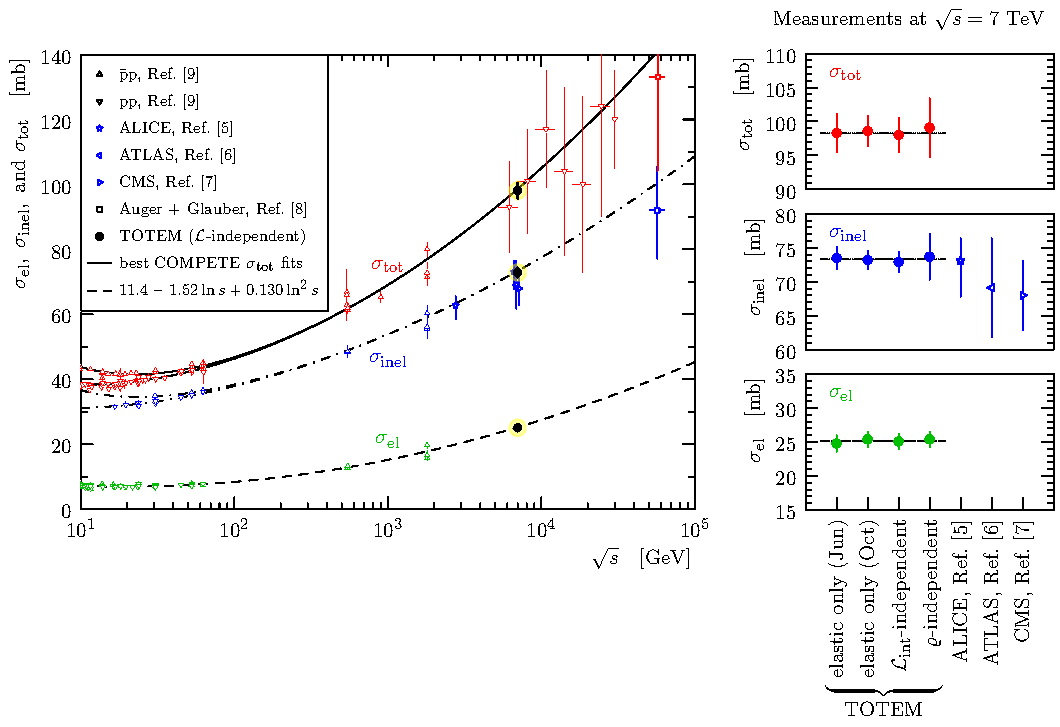
\includegraphics{fig/sigma_tot_el_inel_cmp_big.pdf}
\vskip-5mm
\caption{Left: the dependences of total, inelastic and elastic cross-sections on the scattering energy $\sqrt s$. The continuous black lines (lower for $\rm pp$, upper for $\rm \bar pp$) represent the best fits of the total cross-section data by the COMPETE collaboration \cite{compete}. The dashed line results from a fit of the elastic scattering data. The dash-dotted curves correspond to the inelastic cross-section and were obtained as the difference between the continuous and dashed fits.\hfil\break
Right: measurements of total, inelastic and elastic cross-sections at $\sqrt s = 7\un{TeV}$. The circles represent the four TOTEM measurements summarized in Table~\ref{tab:cs} (weighted mean given by the dotted line), the other points show the measurements of other LHC collaborations.}
\label{fig:cs}
\end{center}
\vskip-10mm
\end{figure*}
}

\def\FigRatio{%
\begin{figure}
\onefigure{fig/sigma_el_to_sigma_tot.pdf}
\vskip-5mm
\caption{The ratio of the elastic to total cross-section as a function of the scattering energy $\sqrt s$. The dashed line shows the ratio of the $\sigma_{\rm el}(s)$ and $\sigma_{\rm tot}(s)$ fits from Figure~\ref{fig:cs}.
}
\label{fig:sigma rat}
\end{figure}
}

%--------------------------------------------------
\section{Introduction}

The TOTEM experiment has recently published \cite{epl96,P1} the differential cross-section for elastic proton-proton scattering as a function of the four-momentum transfer squared, $t$. By extrapolation to $t=0$, the cross-section $\d\sigma_{\rm el}/\d t|_{t=0}$ at the optical point was determined. Integration of the differential distribution yields the elastic cross-section, $\sigma_{\rm el}$. Applying the optical theorem, the total and the fully inclusive inelastic proton-proton cross-sections were derived, with a weak dependence on the $\rho$ parameter (the ratio of the real to the imaginary part of the forward hadronic scattering amplitude):
\begin{equation}
\label{eq:m el}
	\sigma_{\rm tot}^2 = {16\pi\, (\hbar c)^2\over 1 + \rho^2}\, \left. \d\sigma_{\rm el}\over\d t\right|_{t=0}\ ,\qquad
	\sigma_{\rm inel} = \sigma_{\rm tot} - \sigma_{\rm el}\ .
\end{equation}
%The results for the low-luminosity measurement \cite{epl96} and the higher-luminosity measurement \cite{P1} are summarized in Table~\ref{tab:cs}.
All these cross-sections are exclusively based on the measurement of the elastic scattering cross-section.

Moreover, taking advantage of the two trigger-capable forward charged-particle telescopes T1 and T2, the inelastic cross-section was also directly measured \cite{P2} using the same data set as in \cite{P1}. A small Monte-Carlo correction ($\approx 4\%$) was applied to account for the invisible events in the very forward direction $|\eta| > 6.5$, mainly due to low-mass single diffraction. The cross-sections values with their systematic uncertainties are summarized in Table~\ref{tab:cs}.

The excellent agreement between the two completely different measurements of the inelastic cross-sections confirms the understanding of the systematic uncertainties and corrections applied in both methods. Taking maximum advantage of the two measurements by combining them in different ways allows extracting more information from the data, such as:
\begin{itemize}
%\setlength{\partopsep}{0pt}%
%\setlength{\topsep}{0pt}%
\setlength{\itemsep}{-4pt}%
\item luminosity-independent cross-sections,
\item luminosity determination,
\item $\rho$-independent cross-sections,
\item luminosity- and $\rho$-independent cross-section ratios,
\item $\rho$ constraints.
\end{itemize}

The results presented in this article are obtained from the data collected in October 2011 (for details see Table~1 in \cite{P1}). For completeness, some of the results will be compared to those of the lower-luminosity run from June 2011 \cite{epl96}, where only the elastic part of the analysis could be performed.


%--------------------------------------------------
\section{Luminosity independent cross-sections}

Using the optical theorem, one can combine the elastic measurements from \cite{P1} and the inelastic measurements from \cite{P2} to derive the total cross-section without the knowledge of the luminosity:
\begin{equation}
\label{eq:m lumi indep}
	\sigma_{\rm tot} = {16\pi\, (\hbar c)^2\over 1 + \rho^2}\, {\d N_{\rm el}/\d t|_{t=0} \over N_{\rm el} + N_{\rm inel} }\ ,
\end{equation}
where $N_{\rm el}$ and $N_{\rm inel}$ stand for rates integrated over the run period. Taking $\rho = 0.141\pm 0.007$ from the COMPETE extrapolation \cite{compete} yields the luminosity-independent total cross-section, see Table~\ref{tab:cs}. Furthermore, using the measured ratio $N_{\rm el} / N_{\rm inel}$, also the elastic and inelastic cross-sections can be derived independently from the luminosity. These cross-sections are given in Table~\ref{tab:cs} with their uncertainty compositions.

\TabCS
\TabLumi
\FigSigmas

%--------------------------------------------------
\section{Luminosity determination}

The optical theorem can also be applied in a complementary way such that the luminosity is determined:
\begin{equation}
\label{eq:lumi oct}
{\cal L_{\rm int}^{\rm TOTEM}} = {1 + \rho^2 \over 16\pi\, (\hbar c)^2}\, { (N_{\rm el} + N_{\rm inel})^2 \over \d N_{\rm el}/\d t|_{t=0} }\ .
\end{equation}
Thus, integrating the rates over the data-taking period during which the elastic \cite{P1} and inelastic \cite{P2} interactions have independently but simultaneously been measured, the integrated luminosity ${\cal L}_{\rm int}^{\rm TOTEM}$ is obtained. Using the above $\rho$ value, the luminosity determined by TOTEM for the October run is compared in Table~\ref{tab:lumi} to the one obtained by CMS in a completely different way. Both measurements agree well within their uncertainties.


Once the cross-section of a process is known, it can be, in general, used for luminosity determination. In particular, knowing the total and elastic cross-sections, the integrated luminosity of the earlier June run \cite{epl96} has been calculated from the elastic scattering rates $\d N_{\rm el}/\d t|_{t=0}$ and $N_{\rm el}$, which are of course highly correlated:
\begin{equation}
\label{eq:lumi jun tot}
{\cal L}_{\rm int}^{\rm June} =  {16\pi\, (\hbar c)^2\over 1 + \rho^2}\, \left. \d N_{\rm el}^{\rm June}\over\d t\right|_{t=0}\, {1\over \sigma_{\rm tot}^2}\ ,
\end{equation}
\begin{equation}
\label{eq:lumi jun el}
{\cal L}_{\rm int}^{\rm June} = {N_{\rm el}^{\rm June}\over \sigma_{\rm el}}\ .
\end{equation}
The luminosity-independent values for the total and elastic cross-sections (see Table~\ref{tab:cs}) yield the integrated luminosities for the June run, which are again in excellent agreement with the CMS results, see Table~\ref{tab:lumi}.

%--------------------------------------------------
\section{$\rho$-independent quantities}

$\rho$ enters into the equations when the optical theorem is used. However, a $\rho$-independent determination of the total cross-section can be obviously obtained by summing directly the elastic \cite{P1} and inelastic  \cite{P2} cross-sections:
\begin{equation}
\label{eq:m rho indep}
\sigma_{\rm tot} = \sigma_{\rm el} + \sigma_{\rm inel}\ .
\end{equation}
These $\rho$-independent cross-sections (see Table~\ref{tab:cs}) have a larger uncertainty due to the direct propagation of the luminosity uncertainty which, however, cancels for the cross-section ratios
$$
{\sigma_{\rm el} \over \sigma_{\rm inel}} = 0.345 \pm 0.009\ ,\qquad {\sigma_{\rm el}\over \sigma_{\rm tot}} = 0.257 \pm 0.005\ .
$$


%--------------------------------------------------
\section{$\rho$ determination}

The elastic and inelastic measurements can be combined in order to determine $\rho^2$:
\begin{equation}
\label{eq:rho}
\rho^2 = 16\pi\ (\hbar c)^2\ {\cal L_{\rm int}^{\rm CMS}}\ {\d N_{\rm el}/\d t|_{t=0}\over (N_{\rm el} + N_{\rm inel})^2} - 1\ .
\end{equation}
Note that this is a direct measurement at $\sqrt s = 7\un{TeV}$, not an extrapolation from lower-energy measurements. Inserting the values from \cite{P1,P2} and the CMS luminosity measurement yields $\rho^2 = 0.009 \pm 0.056$ (mean and standard deviation). This estimate of $\rho^2$ cannot be translated into terms of $\rho$ in a straight-forward manner since an important part of the $\rho^2$ distribution extends to negative values, where square root is not defined. Instead, one can state that at $95\%$ confidence level $\rho^2 < 0.10$. This upper bound can be equally expressed as $\rho < 0.32$. Alternatively, one can pursue the Bayes' approach to estimate $|\rho|$. Taking a uniform prior $|\rho|$ distribution, it yields a posterior distribution with mean $0.145$ and standard deviation $0.091$.

%--------------------------------------------------
\section{Comparison with other experiments}

The total, elastic and inelastic cross-section values obtained with different methods and data sets (summarized in Table~\ref{tab:cs}) show excellent agreement. In particular, the inelastic cross-sections from two completely independent measurements, once determined from the elastic measurement with the Roman Pot detectors and once directly from the more central charged-particle telescopes, agree remarkably well with each other and also with the ALICE \cite{alice_inel}, ATLAS \cite{atlas_inel} and CMS \cite{cms_inel} results (see Figure~\ref{fig:cs} right).

The energy dependence of the proton-(anti)proton cross-sections is shown in Figure~\ref{fig:cs} left. The best fit of $\sigma_{\rm tot}(s)$ by the COMPETE Collaboration \cite{compete} (published before the TOTEM result) describes the energy dependence well even up to the highest energies measured.  

The ratio $\sigma_{\rm el}/\sigma_{\rm tot}$ can give some insights into the shape and the opacity of the proton, subject to model-dependent theoretical interpretations. The steady rise of this ratio with energy (Figure~\ref{fig:sigma rat}) is often interpreted as the increase of proton size and opacity with energy. 

\FigRatio

%--------------------------------------------------
\section{Relevance for cosmic-ray measurements}

The LHC energy begins to overlap with the energy range where large area cosmic ray showers are studied (see Figure~\ref{fig:cs}). Investigations of high-energy proton-proton interactions at the LHC are therefore of high importance for the study of the development of cosmic ray showers in the atmosphere and thus for high-energy cosmic ray interpretations, like e.g.~the energy spectrum and particle composition \cite{enterria}.  The most important observable is the shower maximum $X_{\rm max}$ which is related to the primary particle mass. It strongly depends on the inelastic $\rm p$-air cross-section. It is worth mentioning that calculations of hadron-nucleus cross-sections in the Glauber-Gribov formalism \cite{nagano,glauber} require the knowledge of not only the inelastic $\rm pp$ cross-section but also the proton-proton elastic scattering amplitude in the small $|t|$-range. The latest Auger measurement of the inelastic cross-section at $\sqrt s = 57\un{TeV}$ \cite{auger} (Figure~\ref{fig:cs}) used the TOTEM cross-section values as an input. In addition, all kinds of diffractive phenomena influence the development of the shower cascade and the multiplicity fluctuations of secondary hadrons. Thus the measurements of the $\rm pp$ cross-sections and the particle flow are of high importance for the interpretation of cosmic ray showers.

%--------------------------------------------------
\section{Final remark}

Within the currently available $|t|$-range and with the present experimental resolution, no effects due to the Coulomb interaction have been observable. Therefore, the obtained elastic scattering $|t|$-distribution has been -- within the experimental uncertainties -- attributed to the hadronic component only, used in the optical theorem. Moreover, a larger-$\beta^*$ optics ($\beta^* = 1000\un{m}$) has been developed. A recent successful run with this optics has demonstrated that $|t|$ values down to $0.0005\un{GeV^2}$ can be attained. A study of the Coulomb-hadronic interference and an observation of the low-$|t|$ hadronic cross-section are, therefore, in reach.

%--------------------------------------------------
%\vskip-3mm
\acknowledgments
%\vskip-3mm

We are indebted to the beam optics development team
%({\sc A.~Verdier} in the initial phase, {\sc H.~Burkhardt}, {\sc G.~M\" uller}, {\sc S.~Redaelli}, {\sc J.~Wenninger}, {\sc S.~M.~White})
for the design, the thorough preparations and the successful commissioning of the $\beta^* = 90\un{m}$ optics. We congratulate the CERN accelerator groups for the very smooth operation in 2011. We thank
%{\sc M.~Ferro-Luzzi}
the LHC physics coordinators for scheduling the dedicated fills.

We are grateful to CMS for providing their luminosity measurements.

We thank S.~Ostapchenko and R.~Ulrich for valuable discussions on the cosmic-ray implications of our results.

This work was supported by the institutions listed on the front page and partially also by NSF (US), the Magnus
Ehrnrooth foundation (Finland), the Waldemar von Frenckell foundation (Finland), the Academy of
Finland, the OTKA grant NK 73143 (Hungary) and the NKTH-OTKA grant 74458 (Hungary).

%--------------------------------------------------
%\vskip-3mm
%\vskip0mm % to cancell the following unskip
\begin{thebibliography}{00}

\bibitem{epl96}
    %First measurements of the total proton-proton cross section at the LHC energy of $\sqrt s =7\,\rm TeV$ CERN-PH-EP-2011-158
	\Name{Antchev G.~{\it et al.}~(TOTEM Collaboration)}
	\REVIEW{Europhys.~Lett.}{96}{2011}{21002}

\bibitem{P1} 
	\Name{Antchev G.~{\it et al.}~(TOTEM Collaboration)}
	CERN-PH-EP-2012-239
	%\REVIEW{Europhys.~Lett.}{TODO}{2012}{TODO}

\bibitem{P2} 
	\Name{Antchev G.~{\it et al.}~(TOTEM Collaboration)}
	{\it  Measurement of proton-proton inelastic scattering cross-section at $\sqrt s = 7\un{TeV}$},
	%CERN-PH-EP-2012-xxx, xxx 2012
	%\REVIEW{Europhys.~Lett.}{XX}{2012}{XXXXX}
	to be published

%\bibitem{epl95}
%    %Proton-proton elastic scattering at the LHC energy of \sqrt{s} = 7 TeV, Europhys. Lett. 95 (2011) 41001,CERN-PH-EP-2011-101 
%	\Name{Antchev G.~{\it et al.}~(TOTEM Collaboration)}
%	\REVIEW{Europhys.~Lett.}{95}{2011}{41001}

%\bibitem{jinst}
%    %The TOTEM Experiment at the CERN Large Hadron Collider, JINST 3 S08007, 2008
%	\Name{Anelli G.~{\it et al.}~(TOTEM Collaboration)}
%	\REVIEW{JINST}{3}{2008}{S08007}

\bibitem{compete} 
	\Name{Cudell~J.~R.~{\it et al.} (COMPETE Collaboration)}
	\REVIEW{Phys.\ Rev.\ Lett.}{89}{2002}{201801}

\bibitem{alice_inel}
%Measurement of inelastic, single- and double-diffraction cross sections in proton-proton collisions at the LHC with ALICE
	\Name{ALICE Collaboration}
	CERN-PH-EP-2012-238

\bibitem{atlas_inel}
%arXiv:1104.0326; CERN-PH-EP-2011-047
%Measurement of the Inelastic Proton-Proton Cross-Section at s√=7 TeV with the ATLAS Detector
	\Name{ATLAS Collaboration}
	\REVIEW{Nature Commun.}{2}{2011}{463}

\bibitem{cms_inel}
	%\Name{Zsigmond, A.~J.~(CMS collaboration)}
	%{\it Inelastic proton-proton cross section measurements in CMS at $\sqrt s = 7\un{TeV}$}, 
	%presented at {\it XX International Workshop on Deep-Inelastic Scattering and Related Subjects}, Bonn, Germany, 26-30 March 2012.
	%arXiv:1205.3142
	\Name{CMS collaboration}
	CMS-PAS-FWD-11-001 and
	CMS-PAS-QCD-11-002
	%CERN-PH-EP-2012-293

\bibitem{auger}
%title = {Measurement of the Proton-Air Cross Section at $\sqrt{s}\mathbf{=}57\text{\,}\text{\,}\mathrm{TeV}$ with the Pierre Auger Observatory},
%url = {http://link.aps.org/doi/10.1103/PhysRevLett.109.062002},
	\Name{Pierre Auger Collaboration}
	\REVIEW{Phys.\ Rev.\ Lett.}{109}{2012}{062002}

\bibitem{pdg} 
	\Name{Nakamura K.~\etal{} (Particle Data Group)}
	\REVIEW{J.~Phys.}{G37}{2010}{075021}

\bibitem{enterria}
	\Name{d'Enterria D.~\etal}
	\REVIEW{Astropart.~Phys.}{35}{2011}{98}

\bibitem{nagano}
	\Name{Nagano M.~and Watson A.~A.}
	\REVIEW{Rev.~Mod.~Phys.}{72}{2000}{689}

\bibitem{glauber}
	\Name{Glauber R.~J.}
	Lectures in Theoretical Physics, ed. by W.~E.~Britten (Interscience, NY,1959) v.1, p. 315

\end{thebibliography}

\end{document}
